% Created by tikzDevice version 0.7.0 on 2015-01-23 00:12:16
% !TEX encoding = UTF-8 Unicode
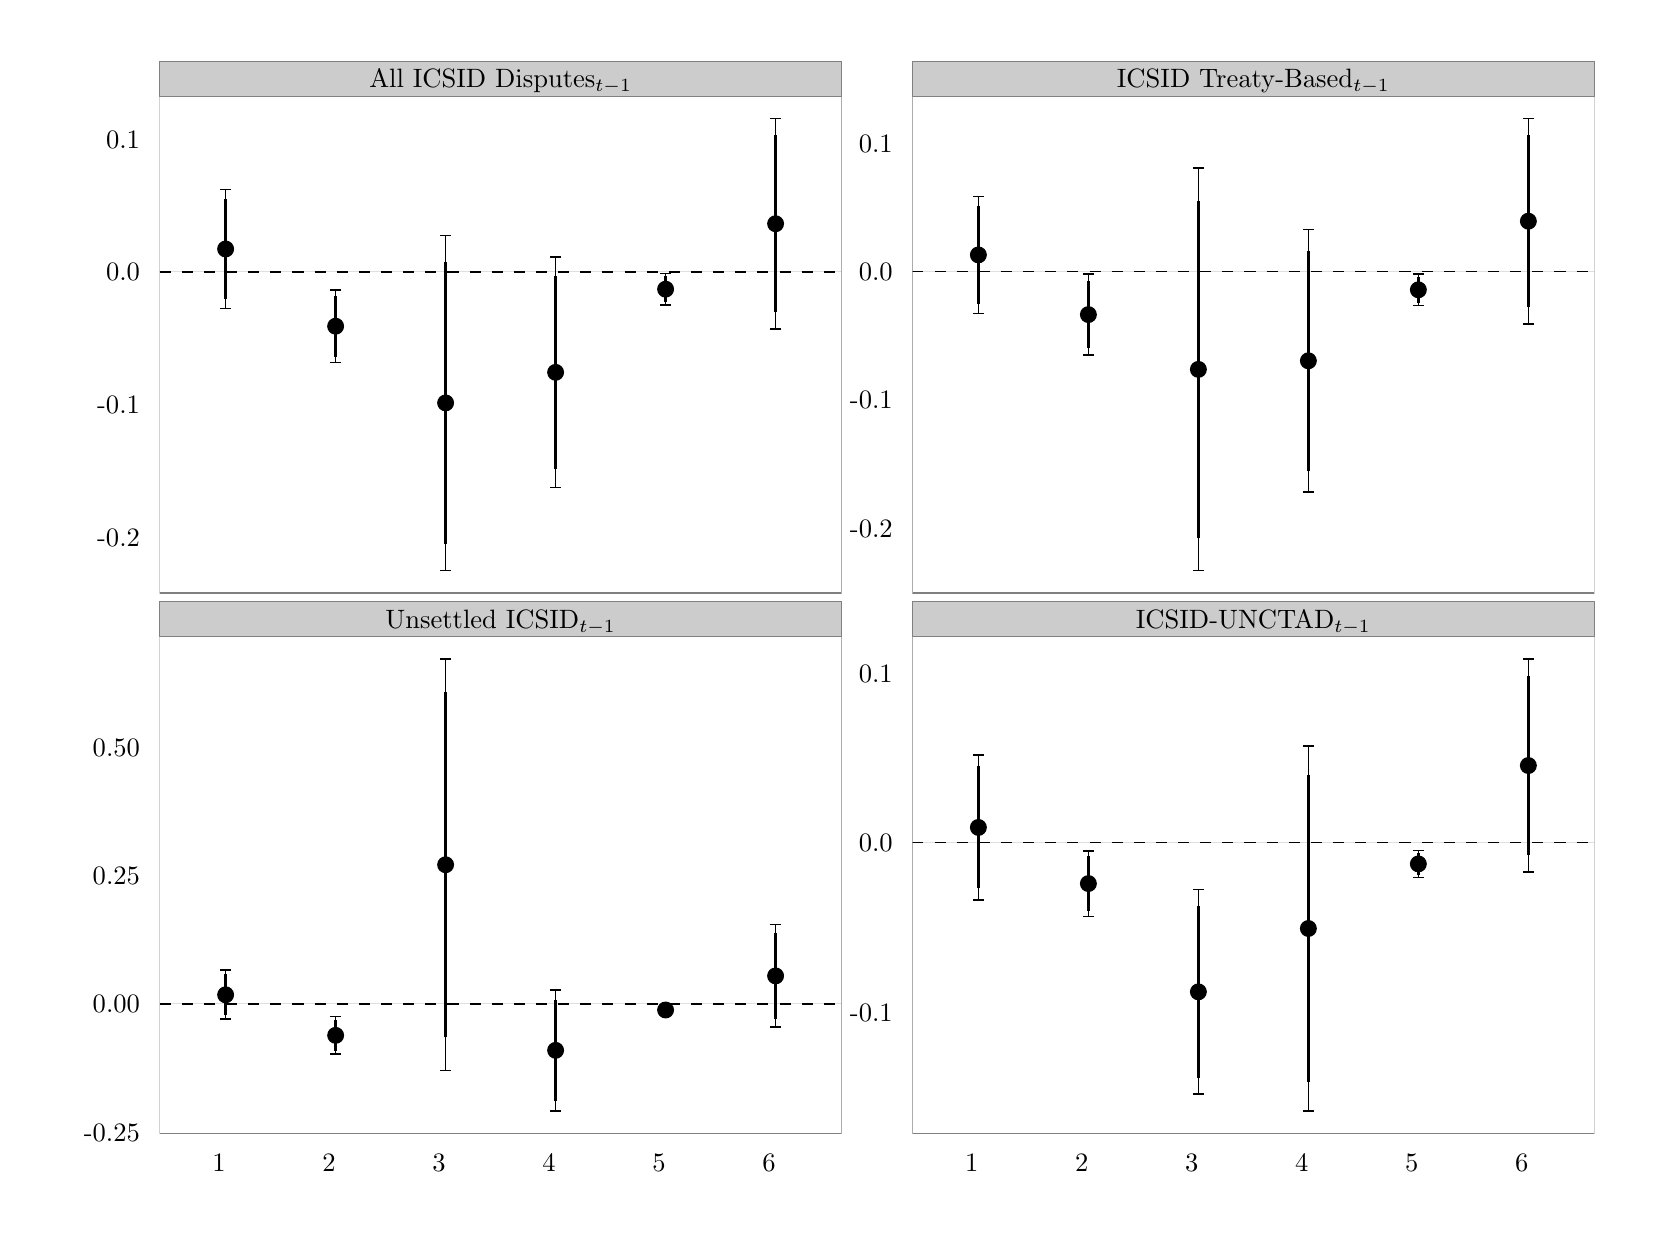
\begin{tikzpicture}[x=1pt,y=1pt]
\definecolor[named]{fillColor}{rgb}{1.00,1.00,1.00}
\path[use as bounding box,fill=fillColor,fill opacity=0.00] (0,0) rectangle (578.16,433.62);
\begin{scope}
\path[clip] (  0.00,  0.00) rectangle (578.16,433.62);
\definecolor[named]{drawColor}{rgb}{1.00,1.00,1.00}
\definecolor[named]{fillColor}{rgb}{1.00,1.00,1.00}

\path[draw=drawColor,line width= 0.6pt,line join=round,line cap=round,fill=fillColor] (  0.00,  0.00) rectangle (578.16,433.62);
\end{scope}
\begin{scope}
\path[clip] ( 47.68,229.31) rectangle (294.11,408.94);
\definecolor[named]{fillColor}{rgb}{1.00,1.00,1.00}

\path[fill=fillColor] ( 47.68,229.31) rectangle (294.11,408.94);
\definecolor[named]{drawColor}{rgb}{0.00,0.00,0.00}
\definecolor[named]{fillColor}{rgb}{0.00,0.00,0.00}

\path[draw=drawColor,draw opacity=0.30,line width= 0.3pt,line join=round,fill=fillColor,fill opacity=0.30] ( 71.53,332.16) -- ( 71.53,375.12);

\path[draw=drawColor,draw opacity=0.30,line width= 0.3pt,line join=round,fill=fillColor,fill opacity=0.30] (111.28,312.60) -- (111.28,338.88);

\path[draw=drawColor,draw opacity=0.30,line width= 0.3pt,line join=round,fill=fillColor,fill opacity=0.30] (151.02,237.48) -- (151.02,358.57);

\path[draw=drawColor,draw opacity=0.30,line width= 0.3pt,line join=round,fill=fillColor,fill opacity=0.30] (190.77,267.44) -- (190.77,350.71);

\path[draw=drawColor,draw opacity=0.30,line width= 0.3pt,line join=round,fill=fillColor,fill opacity=0.30] (230.51,333.46) -- (230.51,344.77);

\path[draw=drawColor,draw opacity=0.30,line width= 0.3pt,line join=round,fill=fillColor,fill opacity=0.30] (270.26,324.76) -- (270.26,400.78);
\definecolor[named]{drawColor}{rgb}{0.00,0.00,0.00}
\definecolor[named]{fillColor}{rgb}{0.00,0.00,0.00}

\path[draw=drawColor,line width= 1.1pt,line join=round,fill=fillColor] ( 71.53,335.62) -- ( 71.53,371.66);

\path[draw=drawColor,line width= 1.1pt,line join=round,fill=fillColor] (111.28,314.71) -- (111.28,336.77);

\path[draw=drawColor,line width= 1.1pt,line join=round,fill=fillColor] (151.02,247.21) -- (151.02,348.84);

\path[draw=drawColor,line width= 1.1pt,line join=round,fill=fillColor] (190.77,274.13) -- (190.77,344.02);

\path[draw=drawColor,line width= 1.1pt,line join=round,fill=fillColor] (230.51,334.37) -- (230.51,343.86);

\path[draw=drawColor,line width= 1.1pt,line join=round,fill=fillColor] (270.26,330.88) -- (270.26,394.67);

\path[draw=drawColor,line width= 0.6pt,dash pattern=on 4pt off 4pt ,line join=round,fill=fillColor] ( 47.68,345.41) -- (294.11,345.41);

\path[draw=drawColor,line width= 0.4pt,line join=round,line cap=round,fill=fillColor] ( 71.53,353.64) circle (  2.85);

\path[draw=drawColor,line width= 0.4pt,line join=round,line cap=round,fill=fillColor] (111.28,325.74) circle (  2.85);

\path[draw=drawColor,line width= 0.4pt,line join=round,line cap=round,fill=fillColor] (151.02,298.02) circle (  2.85);

\path[draw=drawColor,line width= 0.4pt,line join=round,line cap=round,fill=fillColor] (190.77,309.07) circle (  2.85);

\path[draw=drawColor,line width= 0.4pt,line join=round,line cap=round,fill=fillColor] (230.51,339.12) circle (  2.85);

\path[draw=drawColor,line width= 0.4pt,line join=round,line cap=round,fill=fillColor] (270.26,362.77) circle (  2.85);

\path[draw=drawColor,line width= 0.6pt,line join=round] ( 69.54,375.12) --
	( 73.52,375.12);

\path[draw=drawColor,line width= 0.6pt,line join=round] ( 71.53,375.12) --
	( 71.53,332.16);

\path[draw=drawColor,line width= 0.6pt,line join=round] ( 69.54,332.16) --
	( 73.52,332.16);

\path[draw=drawColor,line width= 0.6pt,line join=round] (109.29,338.88) --
	(113.26,338.88);

\path[draw=drawColor,line width= 0.6pt,line join=round] (111.28,338.88) --
	(111.28,312.60);

\path[draw=drawColor,line width= 0.6pt,line join=round] (109.29,312.60) --
	(113.26,312.60);

\path[draw=drawColor,line width= 0.6pt,line join=round] (149.04,358.57) --
	(153.01,358.57);

\path[draw=drawColor,line width= 0.6pt,line join=round] (151.02,358.57) --
	(151.02,237.48);

\path[draw=drawColor,line width= 0.6pt,line join=round] (149.04,237.48) --
	(153.01,237.48);

\path[draw=drawColor,line width= 0.6pt,line join=round] (188.78,350.71) --
	(192.76,350.71);

\path[draw=drawColor,line width= 0.6pt,line join=round] (190.77,350.71) --
	(190.77,267.44);

\path[draw=drawColor,line width= 0.6pt,line join=round] (188.78,267.44) --
	(192.76,267.44);

\path[draw=drawColor,line width= 0.6pt,line join=round] (228.53,344.77) --
	(232.50,344.77);

\path[draw=drawColor,line width= 0.6pt,line join=round] (230.51,344.77) --
	(230.51,333.46);

\path[draw=drawColor,line width= 0.6pt,line join=round] (228.53,333.46) --
	(232.50,333.46);

\path[draw=drawColor,line width= 0.6pt,line join=round] (268.27,400.78) --
	(272.25,400.78);

\path[draw=drawColor,line width= 0.6pt,line join=round] (270.26,400.78) --
	(270.26,324.76);

\path[draw=drawColor,line width= 0.6pt,line join=round] (268.27,324.76) --
	(272.25,324.76);
\definecolor[named]{drawColor}{rgb}{0.50,0.50,0.50}

\path[draw=drawColor,line width= 0.6pt,line join=round,line cap=round] ( 47.68,229.31) rectangle (294.11,408.94);
\end{scope}
\begin{scope}
\path[clip] (319.69,229.31) rectangle (566.12,408.94);
\definecolor[named]{fillColor}{rgb}{1.00,1.00,1.00}

\path[fill=fillColor] (319.69,229.31) rectangle (566.12,408.94);
\definecolor[named]{drawColor}{rgb}{0.00,0.00,0.00}
\definecolor[named]{fillColor}{rgb}{0.00,0.00,0.00}

\path[draw=drawColor,draw opacity=0.30,line width= 0.3pt,line join=round,fill=fillColor,fill opacity=0.30] (343.54,330.36) -- (343.54,372.64);

\path[draw=drawColor,draw opacity=0.30,line width= 0.3pt,line join=round,fill=fillColor,fill opacity=0.30] (383.29,315.38) -- (383.29,344.51);

\path[draw=drawColor,draw opacity=0.30,line width= 0.3pt,line join=round,fill=fillColor,fill opacity=0.30] (423.03,237.48) -- (423.03,382.81);

\path[draw=drawColor,draw opacity=0.30,line width= 0.3pt,line join=round,fill=fillColor,fill opacity=0.30] (462.78,265.78) -- (462.78,360.69);

\path[draw=drawColor,draw opacity=0.30,line width= 0.3pt,line join=round,fill=fillColor,fill opacity=0.30] (502.52,333.17) -- (502.52,344.62);

\path[draw=drawColor,draw opacity=0.30,line width= 0.3pt,line join=round,fill=fillColor,fill opacity=0.30] (542.27,326.60) -- (542.27,400.78);
\definecolor[named]{drawColor}{rgb}{0.00,0.00,0.00}
\definecolor[named]{fillColor}{rgb}{0.00,0.00,0.00}

\path[draw=drawColor,line width= 1.1pt,line join=round,fill=fillColor] (343.54,333.76) -- (343.54,369.24);

\path[draw=drawColor,line width= 1.1pt,line join=round,fill=fillColor] (383.29,317.72) -- (383.29,342.17);

\path[draw=drawColor,line width= 1.1pt,line join=round,fill=fillColor] (423.03,249.16) -- (423.03,371.13);

\path[draw=drawColor,line width= 1.1pt,line join=round,fill=fillColor] (462.78,273.41) -- (462.78,353.06);

\path[draw=drawColor,line width= 1.1pt,line join=round,fill=fillColor] (502.52,334.09) -- (502.52,343.70);

\path[draw=drawColor,line width= 1.1pt,line join=round,fill=fillColor] (542.27,332.57) -- (542.27,394.81);

\path[draw=drawColor,line width= 0.6pt,dash pattern=on 4pt off 4pt ,line join=round,fill=fillColor] (319.69,345.54) -- (566.12,345.54);

\path[draw=drawColor,line width= 0.4pt,line join=round,line cap=round,fill=fillColor] (343.54,351.50) circle (  2.85);

\path[draw=drawColor,line width= 0.4pt,line join=round,line cap=round,fill=fillColor] (383.29,329.94) circle (  2.85);

\path[draw=drawColor,line width= 0.4pt,line join=round,line cap=round,fill=fillColor] (423.03,310.14) circle (  2.85);

\path[draw=drawColor,line width= 0.4pt,line join=round,line cap=round,fill=fillColor] (462.78,313.24) circle (  2.85);

\path[draw=drawColor,line width= 0.4pt,line join=round,line cap=round,fill=fillColor] (502.52,338.89) circle (  2.85);

\path[draw=drawColor,line width= 0.4pt,line join=round,line cap=round,fill=fillColor] (542.27,363.69) circle (  2.85);

\path[draw=drawColor,line width= 0.6pt,line join=round] (341.55,372.64) --
	(345.53,372.64);

\path[draw=drawColor,line width= 0.6pt,line join=round] (343.54,372.64) --
	(343.54,330.36);

\path[draw=drawColor,line width= 0.6pt,line join=round] (341.55,330.36) --
	(345.53,330.36);

\path[draw=drawColor,line width= 0.6pt,line join=round] (381.30,344.51) --
	(385.27,344.51);

\path[draw=drawColor,line width= 0.6pt,line join=round] (383.29,344.51) --
	(383.29,315.38);

\path[draw=drawColor,line width= 0.6pt,line join=round] (381.30,315.38) --
	(385.27,315.38);

\path[draw=drawColor,line width= 0.6pt,line join=round] (421.04,382.81) --
	(425.02,382.81);

\path[draw=drawColor,line width= 0.6pt,line join=round] (423.03,382.81) --
	(423.03,237.48);

\path[draw=drawColor,line width= 0.6pt,line join=round] (421.04,237.48) --
	(425.02,237.48);

\path[draw=drawColor,line width= 0.6pt,line join=round] (460.79,360.69) --
	(464.76,360.69);

\path[draw=drawColor,line width= 0.6pt,line join=round] (462.78,360.69) --
	(462.78,265.78);

\path[draw=drawColor,line width= 0.6pt,line join=round] (460.79,265.78) --
	(464.76,265.78);

\path[draw=drawColor,line width= 0.6pt,line join=round] (500.54,344.62) --
	(504.51,344.62);

\path[draw=drawColor,line width= 0.6pt,line join=round] (502.52,344.62) --
	(502.52,333.17);

\path[draw=drawColor,line width= 0.6pt,line join=round] (500.54,333.17) --
	(504.51,333.17);

\path[draw=drawColor,line width= 0.6pt,line join=round] (540.28,400.78) --
	(544.26,400.78);

\path[draw=drawColor,line width= 0.6pt,line join=round] (542.27,400.78) --
	(542.27,326.60);

\path[draw=drawColor,line width= 0.6pt,line join=round] (540.28,326.60) --
	(544.26,326.60);
\definecolor[named]{drawColor}{rgb}{0.50,0.50,0.50}

\path[draw=drawColor,line width= 0.6pt,line join=round,line cap=round] (319.69,229.31) rectangle (566.12,408.94);
\end{scope}
\begin{scope}
\path[clip] ( 47.68, 34.03) rectangle (294.11,213.66);
\definecolor[named]{fillColor}{rgb}{1.00,1.00,1.00}

\path[fill=fillColor] ( 47.68, 34.03) rectangle (294.11,213.66);
\definecolor[named]{drawColor}{rgb}{0.00,0.00,0.00}
\definecolor[named]{fillColor}{rgb}{0.00,0.00,0.00}

\path[draw=drawColor,draw opacity=0.30,line width= 0.3pt,line join=round,fill=fillColor,fill opacity=0.30] ( 71.53, 75.31) -- ( 71.53, 92.99);

\path[draw=drawColor,draw opacity=0.30,line width= 0.3pt,line join=round,fill=fillColor,fill opacity=0.30] (111.28, 62.73) -- (111.28, 76.25);

\path[draw=drawColor,draw opacity=0.30,line width= 0.3pt,line join=round,fill=fillColor,fill opacity=0.30] (151.02, 56.77) -- (151.02,205.50);

\path[draw=drawColor,draw opacity=0.30,line width= 0.3pt,line join=round,fill=fillColor,fill opacity=0.30] (190.77, 42.20) -- (190.77, 85.95);

\path[draw=drawColor,draw opacity=0.30,line width= 0.3pt,line join=round,fill=fillColor,fill opacity=0.30] (230.51, 76.74) -- (230.51, 80.57);

\path[draw=drawColor,draw opacity=0.30,line width= 0.3pt,line join=round,fill=fillColor,fill opacity=0.30] (270.26, 72.47) -- (270.26,109.49);
\definecolor[named]{drawColor}{rgb}{0.00,0.00,0.00}
\definecolor[named]{fillColor}{rgb}{0.00,0.00,0.00}

\path[draw=drawColor,line width= 1.1pt,line join=round,fill=fillColor] ( 71.53, 76.74) -- ( 71.53, 91.57);

\path[draw=drawColor,line width= 1.1pt,line join=round,fill=fillColor] (111.28, 63.81) -- (111.28, 75.16);

\path[draw=drawColor,line width= 1.1pt,line join=round,fill=fillColor] (151.02, 68.73) -- (151.02,193.54);

\path[draw=drawColor,line width= 1.1pt,line join=round,fill=fillColor] (190.77, 45.72) -- (190.77, 82.43);

\path[draw=drawColor,line width= 1.1pt,line join=round,fill=fillColor] (230.51, 77.05) -- (230.51, 80.27);

\path[draw=drawColor,line width= 1.1pt,line join=round,fill=fillColor] (270.26, 75.45) -- (270.26,106.52);

\path[draw=drawColor,line width= 0.6pt,dash pattern=on 4pt off 4pt ,line join=round,fill=fillColor] ( 47.68, 80.90) -- (294.11, 80.90);

\path[draw=drawColor,line width= 0.4pt,line join=round,line cap=round,fill=fillColor] ( 71.53, 84.15) circle (  2.85);

\path[draw=drawColor,line width= 0.4pt,line join=round,line cap=round,fill=fillColor] (111.28, 69.49) circle (  2.85);

\path[draw=drawColor,line width= 0.4pt,line join=round,line cap=round,fill=fillColor] (151.02,131.14) circle (  2.85);

\path[draw=drawColor,line width= 0.4pt,line join=round,line cap=round,fill=fillColor] (190.77, 64.08) circle (  2.85);

\path[draw=drawColor,line width= 0.4pt,line join=round,line cap=round,fill=fillColor] (230.51, 78.66) circle (  2.85);

\path[draw=drawColor,line width= 0.4pt,line join=round,line cap=round,fill=fillColor] (270.26, 90.98) circle (  2.85);

\path[draw=drawColor,line width= 0.6pt,line join=round] ( 69.54, 92.99) --
	( 73.52, 92.99);

\path[draw=drawColor,line width= 0.6pt,line join=round] ( 71.53, 92.99) --
	( 71.53, 75.31);

\path[draw=drawColor,line width= 0.6pt,line join=round] ( 69.54, 75.31) --
	( 73.52, 75.31);

\path[draw=drawColor,line width= 0.6pt,line join=round] (109.29, 76.25) --
	(113.26, 76.25);

\path[draw=drawColor,line width= 0.6pt,line join=round] (111.28, 76.25) --
	(111.28, 62.73);

\path[draw=drawColor,line width= 0.6pt,line join=round] (109.29, 62.73) --
	(113.26, 62.73);

\path[draw=drawColor,line width= 0.6pt,line join=round] (149.04,205.50) --
	(153.01,205.50);

\path[draw=drawColor,line width= 0.6pt,line join=round] (151.02,205.50) --
	(151.02, 56.77);

\path[draw=drawColor,line width= 0.6pt,line join=round] (149.04, 56.77) --
	(153.01, 56.77);

\path[draw=drawColor,line width= 0.6pt,line join=round] (188.78, 85.95) --
	(192.76, 85.95);

\path[draw=drawColor,line width= 0.6pt,line join=round] (190.77, 85.95) --
	(190.77, 42.20);

\path[draw=drawColor,line width= 0.6pt,line join=round] (188.78, 42.20) --
	(192.76, 42.20);

\path[draw=drawColor,line width= 0.6pt,line join=round] (228.53, 80.57) --
	(232.50, 80.57);

\path[draw=drawColor,line width= 0.6pt,line join=round] (230.51, 80.57) --
	(230.51, 76.74);

\path[draw=drawColor,line width= 0.6pt,line join=round] (228.53, 76.74) --
	(232.50, 76.74);

\path[draw=drawColor,line width= 0.6pt,line join=round] (268.27,109.49) --
	(272.25,109.49);

\path[draw=drawColor,line width= 0.6pt,line join=round] (270.26,109.49) --
	(270.26, 72.47);

\path[draw=drawColor,line width= 0.6pt,line join=round] (268.27, 72.47) --
	(272.25, 72.47);
\definecolor[named]{drawColor}{rgb}{0.50,0.50,0.50}

\path[draw=drawColor,line width= 0.6pt,line join=round,line cap=round] ( 47.68, 34.03) rectangle (294.11,213.66);
\end{scope}
\begin{scope}
\path[clip] (319.69, 34.03) rectangle (566.12,213.66);
\definecolor[named]{fillColor}{rgb}{1.00,1.00,1.00}

\path[fill=fillColor] (319.69, 34.03) rectangle (566.12,213.66);
\definecolor[named]{drawColor}{rgb}{0.00,0.00,0.00}
\definecolor[named]{fillColor}{rgb}{0.00,0.00,0.00}

\path[draw=drawColor,draw opacity=0.30,line width= 0.3pt,line join=round,fill=fillColor,fill opacity=0.30] (343.54,118.34) -- (343.54,170.90);

\path[draw=drawColor,draw opacity=0.30,line width= 0.3pt,line join=round,fill=fillColor,fill opacity=0.30] (383.29,112.50) -- (383.29,136.17);

\path[draw=drawColor,draw opacity=0.30,line width= 0.3pt,line join=round,fill=fillColor,fill opacity=0.30] (423.03, 48.22) -- (423.03,122.22);

\path[draw=drawColor,draw opacity=0.30,line width= 0.3pt,line join=round,fill=fillColor,fill opacity=0.30] (462.78, 42.20) -- (462.78,174.02);

\path[draw=drawColor,draw opacity=0.30,line width= 0.3pt,line join=round,fill=fillColor,fill opacity=0.30] (502.52,126.53) -- (502.52,136.34);

\path[draw=drawColor,draw opacity=0.30,line width= 0.3pt,line join=round,fill=fillColor,fill opacity=0.30] (542.27,128.48) -- (542.27,205.50);
\definecolor[named]{drawColor}{rgb}{0.00,0.00,0.00}
\definecolor[named]{fillColor}{rgb}{0.00,0.00,0.00}

\path[draw=drawColor,line width= 1.1pt,line join=round,fill=fillColor] (343.54,122.57) -- (343.54,166.67);

\path[draw=drawColor,line width= 1.1pt,line join=round,fill=fillColor] (383.29,114.40) -- (383.29,134.27);

\path[draw=drawColor,line width= 1.1pt,line join=round,fill=fillColor] (423.03, 54.17) -- (423.03,116.27);

\path[draw=drawColor,line width= 1.1pt,line join=round,fill=fillColor] (462.78, 52.80) -- (462.78,163.42);

\path[draw=drawColor,line width= 1.1pt,line join=round,fill=fillColor] (502.52,127.32) -- (502.52,135.55);

\path[draw=drawColor,line width= 1.1pt,line join=round,fill=fillColor] (542.27,134.67) -- (542.27,199.31);

\path[draw=drawColor,line width= 0.6pt,dash pattern=on 4pt off 4pt ,line join=round,fill=fillColor] (319.69,139.13) -- (566.12,139.13);

\path[draw=drawColor,line width= 0.4pt,line join=round,line cap=round,fill=fillColor] (343.54,144.62) circle (  2.85);

\path[draw=drawColor,line width= 0.4pt,line join=round,line cap=round,fill=fillColor] (383.29,124.34) circle (  2.85);

\path[draw=drawColor,line width= 0.4pt,line join=round,line cap=round,fill=fillColor] (423.03, 85.22) circle (  2.85);

\path[draw=drawColor,line width= 0.4pt,line join=round,line cap=round,fill=fillColor] (462.78,108.11) circle (  2.85);

\path[draw=drawColor,line width= 0.4pt,line join=round,line cap=round,fill=fillColor] (502.52,131.44) circle (  2.85);

\path[draw=drawColor,line width= 0.4pt,line join=round,line cap=round,fill=fillColor] (542.27,166.99) circle (  2.85);

\path[draw=drawColor,line width= 0.6pt,line join=round] (341.55,170.90) --
	(345.53,170.90);

\path[draw=drawColor,line width= 0.6pt,line join=round] (343.54,170.90) --
	(343.54,118.34);

\path[draw=drawColor,line width= 0.6pt,line join=round] (341.55,118.34) --
	(345.53,118.34);

\path[draw=drawColor,line width= 0.6pt,line join=round] (381.30,136.17) --
	(385.27,136.17);

\path[draw=drawColor,line width= 0.6pt,line join=round] (383.29,136.17) --
	(383.29,112.50);

\path[draw=drawColor,line width= 0.6pt,line join=round] (381.30,112.50) --
	(385.27,112.50);

\path[draw=drawColor,line width= 0.6pt,line join=round] (421.04,122.22) --
	(425.02,122.22);

\path[draw=drawColor,line width= 0.6pt,line join=round] (423.03,122.22) --
	(423.03, 48.22);

\path[draw=drawColor,line width= 0.6pt,line join=round] (421.04, 48.22) --
	(425.02, 48.22);

\path[draw=drawColor,line width= 0.6pt,line join=round] (460.79,174.02) --
	(464.76,174.02);

\path[draw=drawColor,line width= 0.6pt,line join=round] (462.78,174.02) --
	(462.78, 42.20);

\path[draw=drawColor,line width= 0.6pt,line join=round] (460.79, 42.20) --
	(464.76, 42.20);

\path[draw=drawColor,line width= 0.6pt,line join=round] (500.54,136.34) --
	(504.51,136.34);

\path[draw=drawColor,line width= 0.6pt,line join=round] (502.52,136.34) --
	(502.52,126.53);

\path[draw=drawColor,line width= 0.6pt,line join=round] (500.54,126.53) --
	(504.51,126.53);

\path[draw=drawColor,line width= 0.6pt,line join=round] (540.28,205.50) --
	(544.26,205.50);

\path[draw=drawColor,line width= 0.6pt,line join=round] (542.27,205.50) --
	(542.27,128.48);

\path[draw=drawColor,line width= 0.6pt,line join=round] (540.28,128.48) --
	(544.26,128.48);
\definecolor[named]{drawColor}{rgb}{0.50,0.50,0.50}

\path[draw=drawColor,line width= 0.6pt,line join=round,line cap=round] (319.69, 34.03) rectangle (566.12,213.66);
\end{scope}
\begin{scope}
\path[clip] (  0.00,  0.00) rectangle (578.16,433.62);
\definecolor[named]{drawColor}{rgb}{0.50,0.50,0.50}
\definecolor[named]{fillColor}{rgb}{0.80,0.80,0.80}

\path[draw=drawColor,line width= 0.2pt,line join=round,line cap=round,fill=fillColor] ( 47.68,408.94) rectangle (294.11,421.57);
\definecolor[named]{drawColor}{rgb}{0.00,0.00,0.00}

\node[text=drawColor,anchor=base,inner sep=0pt, outer sep=0pt, scale=  0.96] at (170.90,411.95) {All ICSID Disputes$_{t-1}$};
\end{scope}
\begin{scope}
\path[clip] (  0.00,  0.00) rectangle (578.16,433.62);
\definecolor[named]{drawColor}{rgb}{0.50,0.50,0.50}
\definecolor[named]{fillColor}{rgb}{0.80,0.80,0.80}

\path[draw=drawColor,line width= 0.2pt,line join=round,line cap=round,fill=fillColor] (319.69,408.94) rectangle (566.12,421.57);
\definecolor[named]{drawColor}{rgb}{0.00,0.00,0.00}

\node[text=drawColor,anchor=base,inner sep=0pt, outer sep=0pt, scale=  0.96] at (442.90,411.95) {ICSID Treaty-Based$_{t-1}$};
\end{scope}
\begin{scope}
\path[clip] (  0.00,  0.00) rectangle (578.16,433.62);
\definecolor[named]{drawColor}{rgb}{0.50,0.50,0.50}
\definecolor[named]{fillColor}{rgb}{0.80,0.80,0.80}

\path[draw=drawColor,line width= 0.2pt,line join=round,line cap=round,fill=fillColor] ( 47.68,213.66) rectangle (294.11,226.30);
\definecolor[named]{drawColor}{rgb}{0.00,0.00,0.00}

\node[text=drawColor,anchor=base,inner sep=0pt, outer sep=0pt, scale=  0.96] at (170.90,216.68) {Unsettled ICSID$_{t-1}$};
\end{scope}
\begin{scope}
\path[clip] (  0.00,  0.00) rectangle (578.16,433.62);
\definecolor[named]{drawColor}{rgb}{0.50,0.50,0.50}
\definecolor[named]{fillColor}{rgb}{0.80,0.80,0.80}

\path[draw=drawColor,line width= 0.2pt,line join=round,line cap=round,fill=fillColor] (319.69,213.66) rectangle (566.12,226.30);
\definecolor[named]{drawColor}{rgb}{0.00,0.00,0.00}

\node[text=drawColor,anchor=base,inner sep=0pt, outer sep=0pt, scale=  0.96] at (442.90,216.68) {ICSID-UNCTAD$_{t-1}$};
\end{scope}
\begin{scope}
\path[clip] (  0.00,  0.00) rectangle (578.16,433.62);
\definecolor[named]{drawColor}{rgb}{0.00,0.00,0.00}

\node[text=drawColor,anchor=base east,inner sep=0pt, outer sep=0pt, scale=  0.96] at ( 40.57,246.13) {-0.2};

\node[text=drawColor,anchor=base east,inner sep=0pt, outer sep=0pt, scale=  0.96] at ( 40.57,294.12) {-0.1};

\node[text=drawColor,anchor=base east,inner sep=0pt, outer sep=0pt, scale=  0.96] at ( 40.57,342.11) {0.0};

\node[text=drawColor,anchor=base east,inner sep=0pt, outer sep=0pt, scale=  0.96] at ( 40.57,390.09) {0.1};
\end{scope}
\begin{scope}
\path[clip] (  0.00,  0.00) rectangle (578.16,433.62);
\definecolor[named]{drawColor}{rgb}{0.00,0.00,0.00}

\node[text=drawColor,anchor=base east,inner sep=0pt, outer sep=0pt, scale=  0.96] at (312.58,249.43) {-0.2};

\node[text=drawColor,anchor=base east,inner sep=0pt, outer sep=0pt, scale=  0.96] at (312.58,295.83) {-0.1};

\node[text=drawColor,anchor=base east,inner sep=0pt, outer sep=0pt, scale=  0.96] at (312.58,342.24) {0.0};

\node[text=drawColor,anchor=base east,inner sep=0pt, outer sep=0pt, scale=  0.96] at (312.58,388.64) {0.1};
\end{scope}
\begin{scope}
\path[clip] (  0.00,  0.00) rectangle (578.16,433.62);
\definecolor[named]{drawColor}{rgb}{0.00,0.00,0.00}

\node[text=drawColor,anchor=base east,inner sep=0pt, outer sep=0pt, scale=  0.96] at ( 40.57, 31.23) {-0.25};

\node[text=drawColor,anchor=base east,inner sep=0pt, outer sep=0pt, scale=  0.96] at ( 40.57, 77.59) {0.00};

\node[text=drawColor,anchor=base east,inner sep=0pt, outer sep=0pt, scale=  0.96] at ( 40.57,123.96) {0.25};

\node[text=drawColor,anchor=base east,inner sep=0pt, outer sep=0pt, scale=  0.96] at ( 40.57,170.32) {0.50};
\end{scope}
\begin{scope}
\path[clip] (  0.00,  0.00) rectangle (578.16,433.62);
\definecolor[named]{drawColor}{rgb}{0.00,0.00,0.00}

\node[text=drawColor,anchor=base east,inner sep=0pt, outer sep=0pt, scale=  0.96] at (312.58, 74.49) {-0.1};

\node[text=drawColor,anchor=base east,inner sep=0pt, outer sep=0pt, scale=  0.96] at (312.58,135.83) {0.0};

\node[text=drawColor,anchor=base east,inner sep=0pt, outer sep=0pt, scale=  0.96] at (312.58,197.17) {0.1};
\end{scope}
\begin{scope}
\path[clip] (  0.00,  0.00) rectangle (578.16,433.62);
\definecolor[named]{drawColor}{rgb}{0.00,0.00,0.00}

\node[text=drawColor,anchor=base east,inner sep=0pt, outer sep=0pt, scale=  0.96] at ( 71.53, 20.31) {1};

\node[text=drawColor,anchor=base east,inner sep=0pt, outer sep=0pt, scale=  0.96] at (111.28, 20.31) {2};

\node[text=drawColor,anchor=base east,inner sep=0pt, outer sep=0pt, scale=  0.96] at (151.02, 20.31) {3};

\node[text=drawColor,anchor=base east,inner sep=0pt, outer sep=0pt, scale=  0.96] at (190.77, 20.31) {4};

\node[text=drawColor,anchor=base east,inner sep=0pt, outer sep=0pt, scale=  0.96] at (230.51, 20.31) {5};

\node[text=drawColor,anchor=base east,inner sep=0pt, outer sep=0pt, scale=  0.96] at (270.26, 20.31) {6};
\end{scope}
\begin{scope}
\path[clip] (  0.00,  0.00) rectangle (578.16,433.62);
\definecolor[named]{drawColor}{rgb}{0.00,0.00,0.00}

\node[text=drawColor,anchor=base east,inner sep=0pt, outer sep=0pt, scale=  0.96] at (343.54, 20.31) {1};

\node[text=drawColor,anchor=base east,inner sep=0pt, outer sep=0pt, scale=  0.96] at (383.29, 20.31) {2};

\node[text=drawColor,anchor=base east,inner sep=0pt, outer sep=0pt, scale=  0.96] at (423.03, 20.31) {3};

\node[text=drawColor,anchor=base east,inner sep=0pt, outer sep=0pt, scale=  0.96] at (462.78, 20.31) {4};

\node[text=drawColor,anchor=base east,inner sep=0pt, outer sep=0pt, scale=  0.96] at (502.52, 20.31) {5};

\node[text=drawColor,anchor=base east,inner sep=0pt, outer sep=0pt, scale=  0.96] at (542.27, 20.31) {6};
\end{scope}
\end{tikzpicture}
